\documentclass[twoside,openright,a4paper,12pt]{memoir}
\usepackage[utf8]{inputenc}
\usepackage[OT4]{fontenc}
\usepackage{lmodern}
\usepackage[backend=biber,citestyle=authoryear-comp,hyperref=true]{biblatex}
\usepackage{todonotes}
\usepackage{graphicx}
\usepackage{tikz}
\usetikzlibrary{decorations.pathmorphing,backgrounds,positioning,fit}
\usepackage{gensymb}
\usepackage{amsfonts}
\usepackage{amsthm}
\usepackage[version=3,arrows=pgf]{mhchem}
\usepackage{listings}
\usepackage[pdfborder={0,0,0}, colorlinks=true, linkcolor=blue,urlcolor=blue, citecolor=blue]{hyperref}
\usepackage{cleveref}

\addbibresource{bibliography.bib}
\addbibresource{chapters/karstification/karstification.bib}
\addbibresource{chapters/marchingcubes/marchingcubes.bib}

\theoremstyle{definition}
\newtheorem{defn}{Definition}

\lstset{
  language=[ISO]C++,
  breaklines=true,
  basicstyle=\ttfamily
}

\begin{document}
\title{MODELLING SYSTEM OF KARST CAVES FOR COMPUTER GRAPHICS}
\author{Miłosz Kosobucki}

\maketitle
\listoftodos
\newpage

\begin{center}
  \LARGE{Oświadczenie}
\end{center}

Ja, niżej podpisany \textbf{Miłosz Kosobucki} student Wydziału
Matematyki i Informatyki Uniwersytetu im. Adama Mickiewicza w Poznaniu
oświadczam, że przedkładaną pracę dyplomową pt.:

\textbf{Modelling system of karst caves for computer graphics}

napisałem samodzielnie. Oznacza to, że przy pisaniu pracy, poza niezbędnymi
konsultacjami, nie korzystałem z pomocy innych osób, a w szczególności nie
zlecałem opracowania rozprawy lub jej części innym osobom, ani nie
odpisywałem tej rozprawy lub jej części od innych osób.

Oświadczam również, że egzemplarz pracy dyplomowej w formie wydruku
komputerowego jest zgodny z egzemplarzem pracy dyplomowej w formie
elektronicznej.

Jednocześnie przyjmuję do wiadomości, że gdyby powyższe oświadczenie
okazało się nieprawdziwe, decyzja o wydaniu mi dyplomu zostanie cofnięta.

\newcommand{\kropki}[2]{%
  \vbox{%
    \hbox to #1{\dotfill}%
    \vspace{4pt}%
    \hbox to #1{\hss #2\hss}%
  }
}
\vspace{1cm}
\hbox to \textwidth{%
  \hfil
  \kropki{4cm}{data}%
  \hfil\hfil
  \kropki{4cm}{podpis}%
  \hfil
}% \hfil = \hskip 0pt plus 1fil
% \hss = \hskip 0pt plus 1fil minus 1fil
% \hfilneg = \hskip 0pt plus -1fil
\newpage

\begingroup
\footnotesize
\setlength{\parindent}{0pt}
\setlength{\parskip}{\baselineskip}
\copyright 2011 --- 2013 Miłosz Kosobucki \\
All rights reserved
\endgroup

\tableofcontents

\chapter{Introduction}

%This chapter describes motivations behind the development of the thesis. It
%first briefly describes the challenges that arise with ever-increasing capacity
%of computer hardware, that enables nearly photorealistic quality in real-time graphics, but
%at the same time requires enormous amounts of artistic content like models and textures. Procedural
%generation helps to overcome this problem by the usage of parametrized
%algorithms that take limited user input and generate content usually by means
%of randomization or simulation of physical phenomena.
%
%One of such types of content, that may be desirable to generate is a karst cave.
%This geological structure may be an interesting setting for a movie scene or a
%computer game level. At the same time, it is a very complex structure
%that may be time-consuming to model by hand in a way that is both aesthetically
%pleasing and, at least partially, physically correct.

%\section{Advancement of graphics-generation hardware}

%Capabilities of modern computer graphics hardware enables it to


Karst formations are ubiquitous in every continent of Earth. It's estimated that
about 25\% of Earth population depends on drinking water obtained from karst
aquifers \parencite{ford2007karst}. With such profound infulence on human race,
it is essential to know how these geological structures evolve and how they may
react to human activity.

Various simulation models were developed that try to predict how karst aquifers
evolve in time, and how they react to changes in environment. These models are
implemented in computer software and represent simulated karst structure as
net of fractures.

These tools, being aimed at speleogenesis experts, present results of
calculations with simple plots. Programming project of this thesis provides
solution for richer presentation of geometric structure of modelled karst
structure. It can take input data in format that is similar to formats used by
simulation software for results and generate triangle mesh in two file formats,
of which one is simple textual file format importable by most three--dimensional
modelling software.
\section{Structure of the thesis}

\chapter{Karst and karstification process}
\section{Introduction}
%Formation of karst caves is inherently connected with the karst
This chapter will briefly describe karst and processes that govern the
development of karst caves. First, basic definitions are introduced followed by
description of elements of karst landscape and formations. Next, a high level
overview of the karstification process is presented along chemical reactions
in limestone aquifers that are essential in formation of caves. Process and
chemistry of speleothems formation is described at the end of the chapter.
\section{Basics}

\subsection{Definitions}
\begin{description}
  \item[Karstification]
    is not a strictly defined term. Depending on context it may
    mean all forms of corrosion of soluble rocks or it may encompass whole range of
    processes that lead to devolopment of karst formations.
    
    Usually karstification means a landscape forming process that consists of
    dissolution of various kinds of bedrock. The most common kinds of solutes
    are limestone, dolomite, and gypsum \parencite{karstglossary}. However,
    given right conditions even some weathering-resistant rocks like quartzite
    may be subject to karstification \parencite{migon2010}\todo{Check reference}.
    
    Although chemical dissolution is the main driving force behind karstification,
    mechanical forces may also play a role in the final looks of the karst landscape.
    That's why sometimes, all these forces together are put under the umbrella term
    of karstification.

  \item[Karst]
    terrain formation developed throught the means of
    \emph{karstification}. The origin of the term is a German form of Slavic word
    kras or krš meaning bleak, waterless place \parencite{karstglossary}.
  \item[Karst cave]
    hollow space in a karst structure that is large enough for human to enter
    \parencite{hill1997cave}
  \item[Aquifer]
    geological formation that is capable of holding large amounts of water
    through porosity, and other empty spaces inside.
  \item[Recharge]
    process of addition of water to an aquifer.
\end{description}
\subsection{Elements of karst landscape}

\begin{figure}
  \centerline{\includegraphics[width=\textwidth]{chapters/karstification/karst_landscape.jpg}}
  \caption{Karst landscape showing various features of karst aquifers.
    Figure from book by \cite{marshak2006}}
  \label{fig:karstlandscape}
\end{figure}


Karstification process may produce very interesting and varied landscape. Some
of the prominent elements of karst landscapes seen in figure \ref{fig:karstlandscape}
are:

\begin{description}
  \item[Sinkholes]
  \item[Caves]
  \item[Resurgences]
    places where water that went into the aquifer is reemerging to the surface
  \item[Disappearing streams]
  \item[Tunnels]
  \item[Shafts]
\end{description}
\todo{describe each formation}

\section{Overview of the karstification process}

The most important factor in karstification process is flow of solvent throught an
underground aquifer. Since bedrock is subject to geological processes, a
net (sometimes called a matrix) of fractures of varying diameter and shape is
present in it. This solvent, usually water, flows through this kind of net and
reacts with rock in ways described later.

Such karst aquifer may be surrounded on its sides by an aquitard, a substance
that is impenetrable to water.

Water that enters the system may come from precipation, rivers or lakes. Inflow
of water may happen through diffuse infiltration or point infiltration.
Diffuse infiltration happens on larger areas, covered by small fractures whereas
point infiltration requires a prominent fracture to be present in the aquifer
that can take large amounts of water from a river or lake.

Recharge water that comes to the karst aquifer from neighbouring non-karst areas
is called \emph{allogenic recharge}. For example on figure~\ref{fig:karstification}
a river flowing on the upper aquitard and entering the limestone aquifer through
the sinkhole is an allogenic recharge.

On the other hand, recharge water that flows directly to the karst area e.g. by
precipation is called an \emph{autogenic recharge}

Water that flows through the aquifer reacts chemically with walls of the
fractures widening them through dissolution. After going through the aquifer,
water reemerges at lower level through emerging springs or resurgences.

There are also cases of ground formation resulting from human activity.
Although not truly a karst process, a sinkhole that opened in 2010 in city of
Guatemala was a result of combination of loose ground made of volcanic ash and
inadequate draining system, that couldn't dissipate large amounts of water
brought by tropical storm Agatha \parencite{times2010}.

\begin{figure}
  \centerline{\includegraphics[width=\textwidth]{chapters/karstification/karstification.png}}
  \caption{Example of limestone karst aquifer.
    Figure from \cite{golscheider2007methods}}
  \label{fig:karstification}
\end{figure}

\section{Limestone dissolution}

Chemical reactions that take place during the karstification process will be
shown for limestone aquifers. Following description is taken form \cite{dreybrodt2002}
which is based on \cite{plummer1978}.

With the pH of solution at about 7, limestone dissolves through the following
slow reaction:

\begin{equation}
  \cee{H2O + CaCO3 <-> Ca^2 + CO3^2- + H2O}
  \label{eq1}
\end{equation}

Unfortunately, given very weak soulibility of calcium carbonate in water\footnote{Only about 0.0013~g/100~mL in 25\degree C according to \cite{aylward2008si}},
limestone dissolution would be extremely slow.

However, as the rain passes throught the atmosphere, it's picking up carbon
dioxide that gets dissolved in water. Also, top layer of an aquifer, called
\emph{epikarst}, is usually covered by soil that is rich in substances that
contribute with more carbon dioxide. With this aquired \ce{CO2}, small amounts
of carbonic acid are produced:

\begin{equation}
  \cee{H2O + CO2 -> H^+ + HCO3^-}
  \label{eq2}
\end{equation}

Above raction delivers a proton that bonds with carbonate detached during slow
dissolution \ref{eq1}:

\begin{equation}
  \ce{CO3^2- + H^+ -> HCO3^-}
  \label{eq3}
\end{equation}

Thanks to this, the ion activity product \ce{(CO3^2- )} \ce{(Ca^2+)} is below the
solubility constant of calcite. Calcium bicarbonate\footnote{\ce{Ca(HCO3)2}} produced
during this process has orders of magnitude better soulibility in water\footnote{16.6~g/100~mL in 20\degree C according to \cite{aylward2008si}}
what greatly enchances the rate of limestone dissolution.

\Crefrange{eq1}{eq3} can be summed up with the following single
equation:

\begin{equation}
  \ce{CaCO3 + H2O + CO2 -> Ca^2+ + 2HCO3^- }
  \label{eq4}
\end{equation}

\section{Formation of speleothems}

Speleothems are mineral deposits of various kind that form in a process reverse
to dissolution. When water rich in calcium bicarbonate leaves small fissures in
the aquifer and enters big, hollow areas, its pressure lowers and causes
\ce{CO2}-degassing that is the major factor in precipation of calcium carbonate
on the surfaces of caves.

Loss of carbon dioxide leads to supersaturation in the solution reaction that
is directly reverse to reaction \ref{eq4} \parencite{fairchild2012speleothem}:

\begin{equation}
  \ce{Ca^2+ + 2HCO3^- -> CaCO3 + H2O + CO2}
  \label{eq:precipation}
\end{equation}

Water evaporation plays marginal role in speleothem formation, what was shown
by \cite{holland1964cave}\todo{fix bibliography entry}.


\chapter{Previous work}
\section{Ovierview of karstification modelling}
\section{Single fracture simulation}
\section{Two-dimensional simulations}
\section{Three-dimensionsal simulations}
\section{Visualisation techniques}

\chapter{OpenCL heterogenous programming platform}
This chapter will describe OpenCL. A framework for writing applications that
harness computational capabilities of heterogeneous hardware environment on
which applications are run. Since the introduction of programmable pipeline
in GPUs\footnote{Graphics Processing Unit} an opportunity appeared to use
capabilities of these devices to offload highly parallel, computationally
intensive tasks from main CPU\footnote{Central Processing Unit}. OpenCL can also
expose dedicated hardware units designed to perform certain specialized tasks
like Digital Signal Processing.

OpenCL is used in programming project described in \autoref{chap:project}.
Metaballs and Marching Cubes algorithm are implemented with it. Marching Cubes
algorithm and its OpenCL implementation are described in detail in
\autoref{chap:marchingcubes}.
\section{Introduction}
This section is based on \cite{Kirk:2010:PMP:1841511} and
\cite{gaster2012heterogeneous}.

\subsection{Beginnings of programmable GPUs}

From early 1980s to late 1990s most graphic hardware was fixed--function.
I.e. dedicated graphics units exposed fixed set of functions that were
implemented in hardware or drivers. It wasn't possible to write custom program
that would be executed on the GPU.

As the complexity of fixed--function APIs expanded, hardware vendors implemented
them with general purpose processors that could run some limited instruction set
on many processors. This instruction set was used to implement graphics APIs
like OpenGL or DirectX.

In 2001 NVIDIA released GeForce 3 graphics card that exposed this internal
instruction set to users of OpenGL and DirectX APIs. ATI technologies followed
with Radeon 9700 that could also run programs supplied by the user on the GPU.
DirectX 8 and OpenGL introduced programmable vertex stage. With
DirectX 9 another programmable stage was introduced, the pixel (or fragment in
OpenGL terminology) shader. At this point, vertex and pixel shaders were
implemented via separate chips in the GPU. In 2005, with release of XBox 360
first unified architecture was introduced, on which vertex and fragment shaders
were run on the same processor.

Graphics processing, that these devices were build for is very well suited for
parallelization. Vertex shader stage takes list of vertices as its input and
maps them onto the screen optionally defining colour of the vertex. Each
vertex is processed independently making it possible to process many vertices
at the same time.

Pixel shader stage receives position of the point and returns final colour of
the pixel. This also is done independently for each pixel.

\subsubsection[Early attempts at GPGPU]{Early attempts at GPGPU\footnote{General Purpose GPU}}

With the unification of computational resources in the GPUs they started to
resemble highly parallel computers. Researchers noted this fact, and tried to
harness enormous parallel performance for workloads other than graphics.

GPUs of DirectX 9 era were still designed in graphics processing in mind.
Although there were programmable stages in the pipeline, types of input and
output parameters in each stage were severely limited. Moreover, the final
result was generated as a pixel buffer, so the programmer had to map outputs of
his algorithm to 2D screen space with pixel colour as output. Inputs to the
pixel shader stage had to be supplied by textures.

Even with these issues, researchers who managed to port their algorithms to
GPUs reported great performance benefits.

\subsubsection{CUDA}

When working on Tesla GPU architecture, engineers at NVIDIA realized the
potential in providing device's resources in easier way. Additional instructions
and functionalities were added to the device. Among them, read and write
operation with arbitrary offsets\footnote{Shaders could only write to predestined
places in memory, reserved for pixel output}, synchronization barriers for
groups of threads, atomic read/write operations. New parallel programming model
was developed that defined hierarchy of threads.

To expose all these features to programmers new C--like language was
created and named CUDA\footnote{Compute Unified Device Architecture}.

CUDA is capable of operating without any DirectX or OpenGL context. Device it's
run on doesn't even have to be connected to any display output. CUDA programs
are usually inlined in larger C or C++ programs and are called \emph{kernels}.
Special compiler called \emph{nvcc} is used to compile kernel code. For more
information about CUDA refer to official CUDA website\footnote{\url{http://www.nvidia.com/object/cuda_home_new.html}}.

\subsubsection{Inception of OpenCL}

On June 16th, 2008 Khronos Group announced formation of Compute Working Group (CWG)
that was tasked with establishing open standard for programming heterogeneous
CPU and GPU environments\footnote{\url{https://www.khronos.org/news/press/khronos\_launches\_heterogeneous\_computing\_initiative}}.
CWG consisted of many hardware and software vendors interested in
standardization of such API.

Compute Working Group adopted proposal of Apple Inc. that submitted programming
interface called Open Compute Language (OpenCL). Apple was already developing
OpenCL for quite some time to have it ready for its upcoming Mac OS X Snow
Leopard release.

On December 9th, 2008 final specification of OpenCL 1.0 was
released\footnote{\url{https://www.khronos.org/news/press/the\_khronos\_group\_releases\_opencl\_1.0\_specification}}.
Releases of conforming implementations from hardware vendors followed\footnote{http://www.khronos.org/conformance/adopters/conformant-products/\#opencl}.

\subsection{Specification}
OpenCL specification is maintained by the Khronos Group. It consists of C API
and Kernel language that is similar to C99. Khronos releases official C++
wrapper API\footnote{This wrapper API is used in programming project of this thesis}.

Unofficial bindings for various languages and frameworks also exist. Among others
\begin{itemize}
	\item PyOpencl\footnote{\url{http://mathema.tician.de/software/pyopencl}}
		for Python
	\item JOCL\footnote{\url{http://www.jocl.org/}} for Java.
	\item fortrancl\footnote{\url{http://code.google.com/p/fortrancl/}} for Fortran
	\item gocl\footnote{\url{https://github.com/elima/gocl}} wrapper for C
		applications based on GObject
	\item QtOpenCL\footnote{\url{http://doc.qt.digia.com/opencl-snapshot/index.html}}
		wrapper based on Qt library semantics.
\end{itemize}

\section{Logical abstraction of computational resources}

OpenCL aims to be API that lets hardware manufacturers expose various kinds of
devices to the programmers in a consistent and abstracted way. To fulfil this
requirement OpenGL defines logical hierarchy of computational resources.
Hardware vendors map real hardware to this abstraction in their implementations
of OpenCL.

OpenCL defines one processor (\emph{host}) that is coordinating execution of
OpenCL kernels on one or more \emph{devices}. Host, is executing functions from
C API portion of the specification. It's responsible for discovering available
devices, setting up contexts for them, allocating memory on host and devices,
queuing execution of kernels and initiating transfer of data between various
memories.

Diagram of this logical structure is presented in \autoref{fig:clhw}.

\begin{figure}[h]
	\begin{center}
		\includegraphics[scale=0.7]{chapters/opencl/opencl_hwmodel.jpg}
	\end{center}
	\caption{Logical partitioning of hardware in OpenCL}
	\label{fig:clhw}
\end{figure}

\subsection{Platforms}

On the top of the hierarchy is \emph{Platform}. It is usually an implementation
of OpenCL by a single vendor. To query list of available platform in the system
function \texttt{clGetPlatformIds()} must be called twice. Once with parameter
\texttt{platforms} set to \texttt{NULL} to obtain number of platforms, and
second time, with \texttt{platform} parameter set to array that will fit
number of \texttt{cl\_platform\_id} structures equal or greater than the number
in argument \texttt{num\_platforms} retrieved on first invocation of this
function.

Note however, that OpenCL is usually loaded as a dynamic library provided by
vendor. These libraries will usually return only one platform.

To address this problem Khronos Group introduced \texttt{cl\_khr\_icd} extension
that depending on operating system, will look for list of installed OpenCL
ICDs or Installable Client Drivers in place specific for given OS. If
implementation supports this extension, new function \texttt{clIcdGetPlatformIDsKHR}
is available that will present to the user platforms from all vendors available
on the system. This extension also makes sure, that function calls with OpenCL
object created in certain platform will be routed to implementations in this
platform.

\subsection{Devices}

Platform, may contain one or more \emph{devices}. Devices are units that
actually execute the kernel code. Device may map for example to single GPU or
CPU.

For example, NVIDIA OpenCL implementation presents each GPU available in the
system as separate device. OpenCL from AMD besides presenting GPUs also presents
supported CPUs as devices.

Device is last entity in hierarchy that has its distinct API object. Further
elements cannot be operated on, and are just abstract concepts to which vendors
map their hardware.

These elements are \emph{compute units} which are comprised of \emph{processing
elements}. Devices can be queried for number of compute units they contain
through \texttt{clGetDeviceInfo()} function.

\subsubsection{Mapping physical devices to logical hierarchy}

Exact details of mapping is dependant on OpenCL vendor. Underlying architectures
of GPUs, CPUs and DSPs\footnote{Digital Singal Processors} can differ greatly
even within the same class of devices.

\section{Memory types}

\section{Execution model}

\chapter{Isosurface extraction with Marching Cubes}

This chapter will present a method of isosurface extraction that is later used
in the programming project. First, basic definitions will be established and
rationale for generating graphics with volumetric data will be discussed.
Next, brief history and high level overview of Marching Cubes will be presented.
Technical details will follow with description of implementation on highly
parallel GPGPU systems with OpenCL.

\section{Definitions}

\begin{defn}[Density function]
\label{def:density function}
Scalar function
$\mathbb{R}^3\rightarrow\mathbb{R}$ or $\mathbb{R}^2\rightarrow\mathbb{R}$
that defines value of some magnitude in a continuous space. An example of such
function in 3D space is temperature defined in each point in the space. Height
on a flat map on the other hand is a density function in 2D space.
\end{defn}

\begin{defn}[Isosurface]
Surface in three-dimensional space that consists of points that have certain
value of \emph{density function}.
\end{defn}

\begin{defn}[Isovalue]
Certain value of density function which will be considered the surface. Points
in domain which density function value is below this value are considered to
lie below the surface and points which density function value is above this
value are considered to lie above the surface. Points which density function
value equals isovalue are considered to lie exactly on the isosurface.
\end{defn}

\section{Rationale for isosurface rendering}

There are many applications which yield data as a density function. Some of them
are listed below:
\begin{description}
	\item[CT\footnotemark scan.]\footnotetext{Computer Tomography}
		Result of such scan is a discrete lattice of points with certain
		values on vertices
	\item[Weather data]
		Weather data, especially coming from weather models consists of
		scalar values of various parameters (temperature, humidity, etc.)
		on earth's surface
	\item[Arbitrary mathematical function]
		It's often desirable to visualise mathematical function with
		multiple parameters on 2D and 3D plots. For example for
		educational purposes.
	\item[Procedural models]
		Surfaces expressed by density function may be a source of
		visually interesting models that could be hard to model by hand.
\end{description}

Interactive presentation of such data may be very helpful while working with
these applications. Ability to rotate, zoom and scale such surfaces may be
beneficial to understanding the data since human sight apparatus is naturally
well equipped to process 3D objects and images.

\section{Marching Cubes algorithm overview}
\subsection{History \parencite{mchist}}
Marching Cubes algorithm was invented in 1984 by William E. Lorensen and Harvey
E. Cline. While being employed by General Electric they attended a seminar by
GE's Medical Systems Business Group employee Carl Crawford. Mr Crawford
described capabilities of the upcoming rendering engine called \emph{Graphicon},
that rendered using polygons. He also challenged seminar attendees to find
interesting usages for the device. Within a day Lorenson and Cline devised an
algorithm that read volumetric medical data (essentially a density function) and
produced triangle mesh representing isosurface.

General Electric submitted a patent application for the algorithm on
June~5, 1985, which was granted on December~1, 1987 \parencite{mcpatent}.

Partly due to existence of this patent, another algorithm for isosurface
extraction called \emph{Marching Tetrahedra} was invented to give graphics
community method that is not encumbered by patents. \emph{Marching Tetrahedra}
also solves some ambiguities that are present in \emph{Marching Cubes}.

Patent on \emph{Marching Cubes} algorithm expired in 2005.

\subsection{Algorithm description \parencite{Lorensen:1987:MCH:37402.37422}}

Marching cubes algorithm divides space on which it operates into a discrete
lattice of cubes. For each cube, density function value is retrieved for each
vertex of the cube. Density function may be calculated from the position of the
vertex on the fly if it's defined as a mathematical function, or it may be
extracted from some external volumetric data source (e.g. result of CT scan).

Next, for each edge of the cube it's determine whether value at given vertex is
larger or smaller than requested isovalue. If the value on the vertex is smaller
than the threshold isovalue, vertex is below the surface. Otherwise it's above
it.

Being above or below the surface will be called the \emph{sign} of the vertex.
If vertices on the ends of given cube's edge are of different signes, than it's
certain that the surface crosses the edge.

For each cube, there are $2^8=256$ possible combinations of sings of the
vertices. Combination of the cube is called an \emph{index} of this cube.

When the index of the cube is known, pre-generated LUTs\footnote{Look-Up Tables}
are consulted to determine how many polygons and in what configuration should be
emitted for this cube.

Process is repeated for all cubes in the lattice emitted polygons are the output
of the algorithm.

\subsubsection{Cube indexing}

Operation on a single cube begins with evaluating density function on each
vertex of the cube.

Index of the vertex is calculated through operation described below
Figure~\ref{fig:mcnumbering}.

\begin{figure}
  \centerline{
   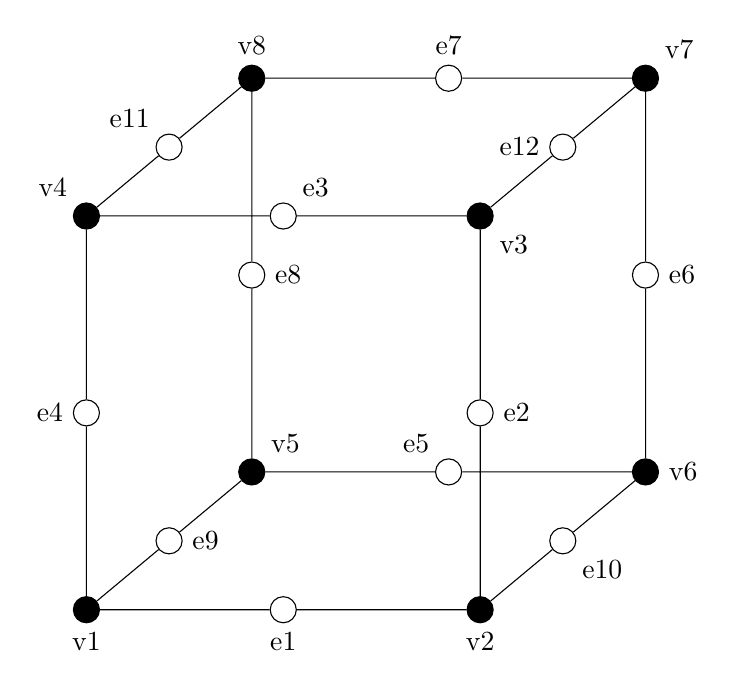
\begin{tikzpicture}[
  z={(-0.42cm,-0.35cm)}, scale=2.5,
  vert/.style={circle,draw=black,fill=black},
  edge/.style={circle,draw=black,fill=white}
]
 
  \node at (0,0,0) [vert,label=below:v1] (v1) {};
  \node at (1,0,0) [edge,label=below:e1] (e1) {};
  \node at (2,0,0) [vert,label=below:v2] (v2) {};
  \node at (2,1,0) [edge,label=right:e2] (e2) {};
  \node at (2,2,0) [vert,label=south east:v3] (v3) {};
  \node at (1,2,0) [edge,label=north east:e3] (e3) {};
  \node at (0,2,0) [vert,label=north west:v4] (v4) {};
  \node at (0,1,0) [edge,label=left:e4] (e4) {};
  \node at (0,0,-2) [vert,label=north east:v5] (v5) {};
  \node at (1,0,-2) [edge,label=north west:e5] (e5) {};
  \node at (2,0,-2) [vert,label=right:v6] (v6) {};
  \node at (2,1,-2) [edge,label=right:e6] (e6) {};
  \node at (2,2,-2) [vert,label=north east:v7] (v7) {};
  \node at (1,2,-2) [edge,label=above:e7] (e7) {};
  \node at (0,2,-2) [vert,label=above:v8] (v8) {};
  \node at (0,1,-2) [edge,label=right:e8] (e8) {};
  \node at (0,0,-1) [edge,label=right:e9] (e9) {};
  \node at (2,0,-1) [edge,label=south east:e10] (e10) {};
  \node at (2,2,-1) [edge,label=left:e12] (e12) {};
  \node at (0,2,-1) [edge,label=north west:e11] (e11) {};

  \draw
    (v1) -- (e1) -- (v2) -- (e2) -- (v3) -- (e3) -- (v4) -- (e4) -- (v1)
    (v5) -- (e5) -- (v6) -- (e6) -- (v7) -- (e7) -- (v8) -- (e8) -- (v5)
    (v1) -- (e9) -- (v5)
    (v2) -- (e10) -- (v6)
    (v4) -- (e11) -- (v8)
    (v3) -- (e12) -- (v7);
\end{tikzpicture}

  }
  \caption{
    Numbering of vertices and edges in Marching Cubes. Cube index is
    derived by concatenation of bits \texttt{index = v8|v7|v6|v5|v4|v3|v2|v1}
    where each \texttt{vi} is logical result (0 or 1) of operation of comparing
    density function value at \emph{i}-th vertex with threshold value
    (\texttt{value(i) > threshold}).
  }
  \label{fig:mcnumbering}
\end{figure}

\subsubsection{Emitting polygons}

When index of the cube is known, LUT is consulted that maps index to list of
edges on which vertex in given cube must be emitted.
\pagebreak
\begin{lstlisting}[caption={Index to edge list LUT. Notice that for indices 0
and 255 no geometry is emitted}]
unsigned char mcTriangleTable[256][16] = {
        {255, 255, 255, 255, 255, 255, 255, 255, 255, 255, 255, 255, 255, 255, 255, 255},
        {0, 8, 3, 255, 255, 255, 255, 255, 255, 255, 255, 255, 255, 255, 255, 255},
        ...
        {0, 3, 8, 255, 255, 255, 255, 255, 255, 255, 255, 255, 255, 255, 255, 255},
        {255, 255, 255, 255, 255, 255, 255, 255, 255, 255, 255, 255, 255, 255, 255, 255}
};
\end{lstlisting}

For each edge on the list vertex is emitted between its two ends in place
proportional to the linear interpolation of density function at the vertices.

Each three vertices form a polygon. In the listing above, value 255 marks an end
of the list for given index.

Next, each polygon is saved in a list for later usage, or directly fed to
rendering device.


\begin{figure}
  \centerline{
    \begin{tikzpicture}[z={(-0.58cm,-0.28cm)}, scale=1.5]
    \input{chapters/marchingcubes/cases.tex}
    \end{tikzpicture}
  }
  \caption{
    All cases in traditional Marching cubes algorithm. Vertices with density
    function above threshold value have black circles on them. Symmetries,
    rotations, and complementary cases (with exception of cases 0 and 255) were
    omitted for brevity.
  }
  \label{fig:mccases}
\end{figure}

\section{Implementation on GPU with OpenCL}
\subsection{Parallel prefix sum operation}

\chapter{Programming project description}
\label{chap:project}
\section{Introduction}

Programming project of this thesis is a set of command line programs, collectively
called \emph{karstgen}, that take
the description of karst cave fracture net and generate polygon mesh in
simple and popular Wavefront OBJ textual file format\footnote{\url{http://www.martinreddy.net/gfx/3d/OBJ.spec}}.

Models created this way may be opened in 3D editing program for further editing
and examination.

Karstgen can also create models for \emph{Vorticity} game engine that was created
by the author together with mr Michał Siejak for graphics related courses\footnote{Computer
  Graphics and Visualiation, summer semester 2009/2009 and Group Project, summer
semester 2009/2010} during licenciate studies at Adam Mickiewicz University of~Poznań.

\section{Architecture}

Karstgen was created with Unix Philosophy in mind \parencite{raymond2003art}.
It is made of two programs named \emph{blobber} and \emph{mcblob} that have
clearly defined responsibilities and communicate through simple textual data
format.  Both programs may take input either from files or from standard input
so they can be piped together with shell pipes. Data flow of karstgen is
presented in \autoref{fig:karstgenflow}.
\begin{figure}[ht]
  \begin{center}
    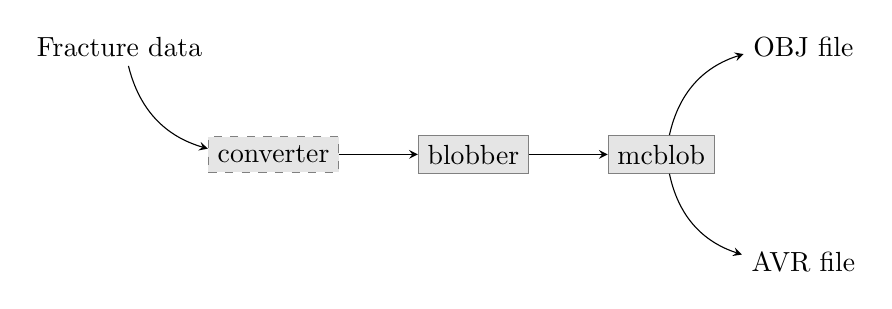
\begin{tikzpicture}[ >=stealth,
provided/.style={rectangle,draw=black!50,fill=black!10},
optional/.style={dashed,rectangle,draw=black!50,fill=black!10}
]

\node (data) {Fracture data};
\node (dummy1) [below=of data] {} ;
\node[optional] (converter) [right=of dummy1] {converter};
\node[provided] (blobber) [right=of converter] {blobber};
\node[provided] (mcblob) [right=of blobber] {mcblob};
\node (dummy) [right=of mcblob] {};
\node (obj) [above=of dummy] {OBJ file};
\node (avr) [below=of dummy] {AVR file};

\draw[->] (data) to [bend right] (converter);
\draw[->] (converter) to (blobber);
\draw[->] (blobber) to (mcblob);
\draw[->] (mcblob) to [bend left](obj);
\draw[->] (mcblob) to [bend right](avr);
\end{tikzpicture}
  \end{center}
  \caption{Data flow of karstgen program. Converter part is required when fracture
  net description is other than expected by blobber.}
  \label{fig:karstgenflow}
\end{figure}

\subsection{Blobber}
Blobber takes description of a fracture net in a simple textual format and
generates list of metaballs (see \autoref{sub:metaballs}). It can
optionally tilt positions and sizes of metaballs in random but adjustable manner
for more natural--looking results. Blobber also controls quality of the final
geometry. For information about runtime parameters invoke:
\begin{verbatim}
./blobber --help
\end{verbatim}

\subsection{Mcblob}
Output generated by blobber is consumed by program named \emph{mcblob}\footnote{\textbf{M}arching
\textbf{C}ubes from \textbf{blob}s} which is general purpose tool that may be used to
generate geometry from a list of metaballs in 3D space through OpenCL--accelerated
 Marching Cubes algorithm.

\section{Implementation details}
\subsection{Metaballs}
Implementation heavily relies on rendering with metaballs. Metaball in 3D space
is a scalar function in the form \parencite[p. 4]{Blinn:1982:GAS:357306.357310}:
\begin{equation}
  f(x,y,z)=Te^{\frac{B}{R^2}r^2 - B}
  \label{eq:metaball}
\end{equation}
where $r$ is distance from point $(x,y,z)$ to the centre of the metaball, $B$ is
,,blobiness'' factor that controls tendency to ,,melt'' with other metaballs, $T$
is isovalue that will be used for rendering and $R$ is the radius of the
metaball if it was isolated from other blobs. This equation is basically a
Gaussian bump with expected value in the middle of the metaball.

If more than one metaball is present in the scene, density function (see Definition
\autoref{def:density function})
is in the form:
\begin{equation}
  d(x,y,z) = \sum_{i=0}^{n} f_i(x,y,z)
  \label{eq:metaballdensity}
\end{equation}
where $n$ is the total number of metaballs in the scene and $f_i$ is function~\ref{eq:metaball}
of the $i$-th metaball.

Metaballs were discovered by Jim Blinn during his work on visualisation of
molecular structures \parencite{Blinn:1982:GAS:357306.357310}. Density function 
was derived from equation defining density of electron field of hydrogen atom
as used in quantum mechanics.

This ,,melting'' property visible when metaballs are close to each other gives
somewhat ,,organic'' look and feel of structures generated with them
(see \autoref{fig:metaballs}).
\label{sub:metaballs}
\begin{figure}[htb]
  \begin{center}
    \includegraphics[width=\textwidth]{chapters/project/metaballs.png}
  \end{center}
  \caption{Two metaballs at various distances showing how they are ,,melting''
    together when getting closer to each other. Geometry was generated with
    \emph{mcblob} program and final image was rendered with Blender 2.68 with
    Cycles renderer. Input file for mcblob that generates this model is
    included with the thesis in file \texttt{fig\_metaballs.in} in kartsgen examples.
  }
  \label{fig:metaballs}
\end{figure}


\subsection{Overview}
Both blobber and mcblob are implemented in C++ language with latest C++11
version of the standard. Build system used to compile the code is \emph{CMake}\footnote{Cross--platform make}
-- meta build system that can generate native projects for various IDEs\footnote{Integrated Development Environment}
and actual build systems. Executables use \emph{Boost Program Options} library
for parsing command line arguments and providing help.

Karstgen uses unit testing framework \emph{Google~Test}\footnote{\url{http://code.google.com/p/googletest/}}.
Documentation is automatically generated from sources with Doxygen
tool.


\subsection{Blobber}

For vector data structures blobber uses \emph{GLM}\footnote{\url{http://glm.g-truc.net/0.9.4/index.html}}
-- a mathematical library that resembles GLSL\footnote{OpenGL Shading Language}.

It reads information about diameters of fractures in fractures network
and places blobs along these fractures with diameters roughly the same as of
these fractures.

Blobber works on data structure named \texttt{DataPoint}:

\begin{lstlisting}
struct DataPoint
{
  	int x, y, z;
	float midDiam;
	std::vector<float> xData;
	std::vector<float> yData;
	std::vector<float> zData;
};
\end{lstlisting}

This structure can describe three fractures originating in index $(x,y,z)$ in
the fracture net and going along each axe in ascending direction. Each fracture
is described as a vector of uniformly distributed diameters. If there is only
one diameter in a vector it is assumed that the fraction it represents has the
same diameter along its whole length. When no diameters are present in some
vector, it is assumed that there is no fracture in this direction.
Additional field \texttt{midDiam} is a diameter of blob that should be placed in
the intersection of the three fractures (see \autoref{fig:datapoint}).

\begin{figure}[hbp]
  \begin{center}
    \begin{tikzpicture}[>=stealth, z={(-0.55cm, -0.33cm)}]

\draw[->,color=green] (0,0,0) -- (0,0,-1) node[font=\tiny,anchor=south west] {$z$};
\draw[->,color=red] (0,0,0) -- (1,0,0) node[font=\tiny,anchor=west] {$x$};
\draw[->,color=blue] (0,0,0) -- (0,-1,0) node[font=\tiny,anchor=north] {$y$};

\draw[fill] (1,-1) circle (0.1);

\draw (1,-1) -- ++(0,0,-5) node[font=\tiny,anchor=south west] {zData};
\draw[fill=white] (0,0)
\foreach \x in {1,2}
{
  (1,-1,-5/3 * \x) circle (0.1)
};

\draw (1,-1) -- ++(5,0,0) node[font=\tiny, anchor=west] {xData};
\draw[fill=white] (1,-1)
\foreach \x in {1,...,4}
{
  ++(1,0,0) circle (0.1)
};

\draw (1,-1) -- ++(0,-5,0) node[font=\tiny,anchor=north] {yData};
\draw[fill=white] (1,-1)
\foreach \x in {1,...,8}
{
  ++(0,-5/9,0) circle (0.1)
};

\draw[fill] (4,-4) circle (0.1) node[anchor=west,xshift=4,yshift=0.8] {-- diameter at intersection};
\draw[fill=white] (4,-5) circle (0.1) node[anchor=west,xshift=4,yshift=-0.5] {-- diameters along fractures};

\end{tikzpicture}
  \end{center}
  \caption{Graphical representation of \texttt{DataPoint} -- a basic structure that
blobber works on. In this example, there are 4 diameters in x direction,
2 in z direction and 8 in y direction.}
  \label{fig:datapoint}
\end{figure}
\pagebreak
Data points are packed into a structure representing whole fracture network
called \texttt{FractureNet}:
\begin{lstlisting}[label={lst:fracturenet},escapeinside={@}{@}]
struct FractureNet
{
	//size of net in number of dataPoints
	int x; int y; int z;
	
	//length of single fracture in each direction
	float xLen; float yLen; float zLen;
	
	std::map<std::tuple<int, int, int>, DataPoint> dataPoints;
};
\end{lstlisting}

Since fracture net is usually quite sparse, dictionary structure\footnote{\texttt{std::map} from C++'s Standard Template Library}
is used to store data points instead of array or vector. Keys in this dictionary
are tuples containing 3D index in a fracture net. This way, given one data point
it is easy to find its neighbours.

\subsubsection{Placement of blobs}

Blobber works on one data point at a time through \texttt{blobs\-From\-Data\-Point()}
function. First, one point is placed in the intersection of the axes with
diameter equal to \texttt{mid\-Point\-Diam}. Then, vector for each non--empty
axe is processed by \texttt{blobsOnVector()} function. Besides the vector of
diameters, this function takes \texttt{midPointDiam} of the data point, and optionally
\texttt{nextDpMidDiam} which is \texttt{midPointDiam} of the next data point
along this axis if such data point exists. Fast lookup of next data point
is possible thanks to dictionary storage of data points. If there is no neighbour data
point at the end of the axis, \texttt{nextDpMidDiam} is considered to be 0.\todo{test if this makes sense}

\begin{figure}[htb]
  \begin{center}
    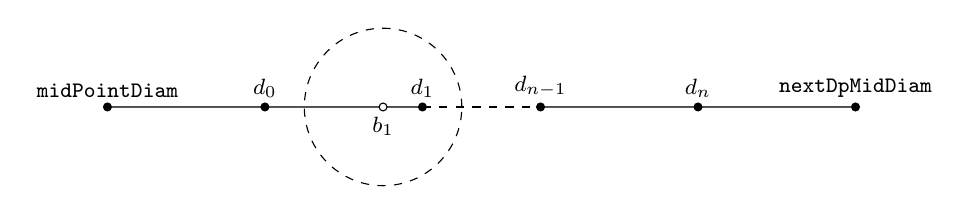
\begin{tikzpicture}[]

\draw (0,0) node [font=\footnotesize,anchor=south] {\texttt{midPointDiam}}
  [fill] circle (0.05) -- ++(2,0)
  circle (0.05) node[font=\footnotesize, anchor=south] {$d_0$}
  -- ++(2.0,0) [fill] circle (0.05) node[font=\footnotesize,anchor=south]{$d_1$};
\draw[dashed] (4,0) -- ++(1.5,0);
\draw[fill] (5.5,0) circle (0.05) node[font=\footnotesize,anchor=south] {$d_{n-1}$}
 -- ++(2,0) node[font=\footnotesize,anchor=south] {$d_{n}$} circle (0.05)
 -- ++(2,0) node[font=\footnotesize,anchor=south] {\texttt{nextDpMidDiam}} circle (0.05);
\draw[dashed]  (3.5,0) circle (1.0);
\draw (3.5,0) [fill=white] circle (0.05) node [font=\footnotesize,anchor=north]{$b_1$};
\end{tikzpicture}
  \end{center}
  \caption{Blobs are placed along fracture defined as set of diameters
    $(d_0,d_1,\cdots,d_{n-1})$. In this example diameter of blob $b_1$ will be a
    linear interpolation of diameters $d_0$ and $d_1$ proportional to distance
    from these diameters.}
  \label{fig:placement}
\end{figure}

Function \texttt{blobsOnVector()} places blobs on the fracture line until
it's fully covered. Diameters of blobs are determined in a way described
in \autoref{fig:placement}.

Format of the input to blobber is described in generated documentation:
\begin{lstlisting}[language=bash,numbers=none]
\doc\blobber\html\index.html
\end{lstlisting}

Output format is the same as input format of mcblob program and is described in
its help:
\begin{lstlisting}[language=bash,numbers=none]
./mcblob --help
\end{lstlisting}

\subsection{Mcblob}
\label{sub:mcblob}

Mcblob uses OpenCL (\autoref{chap:cl}) to calculate density function from
list of blobs provided in input, generates polygon mesh of isosurface
definded by this function using Marching Cubes algorithm (\autoref{chap:marchingcubes})
accelerated with OpenCL and saves results to file in one of two formats.

Bounds of 3D space within which geometry will be generated is defined in input.
It's divided into blocks which are worked on one at a time. For each block,
density function is calculated from blobs, followed by generating geometry.

Finally, when geometry from all blocks is calculated, mcblob writes output to
disk in one of two supported formats.

\subsubsection{Calculating density function}

Each block of voxels is kept by mcblob in a class called \texttt{Grid}. It
contains values of density function on the vertices of the cubes in a block.
These values are stored as one--dimensional array, that is transferable between host and
device memory. If numbers of voxels on axes $x$, $y$ and $z$ are $v_x$, $v_y$
and $v_z$ respectively, \texttt{Grid} will store 1D array
of \texttt{float4} values that is $(v_x+1)\times(v_y+1)\times(v_z+1)$ elements long.

\begin{figure}[tb]
  \begin{center}
    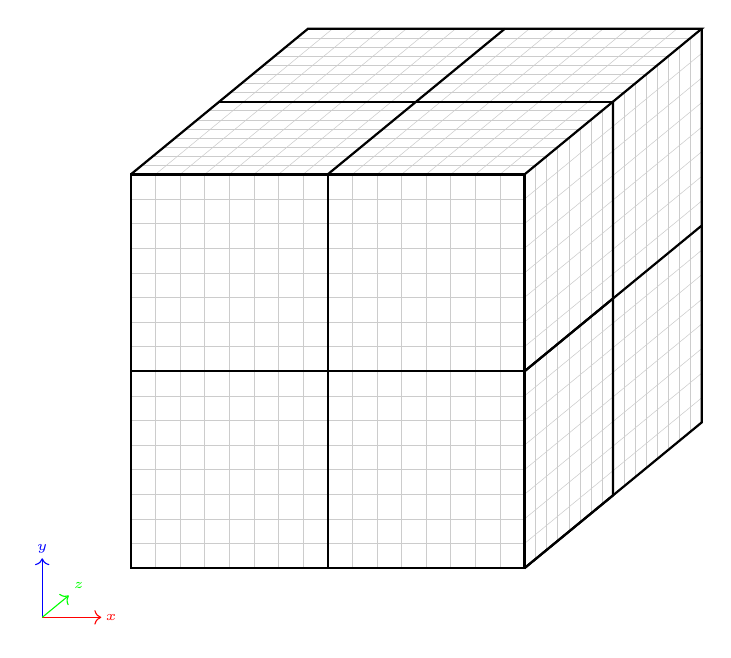
\begin{tikzpicture}[z={(-0.45cm,-0.37cm)}, scale=2.5]

\tikzstyle{inner} = [gray!40!white,very thin]
%front face vertical
\foreach \x in {1,2,3,4,5,6,7,9,10,11,12,13,14,15}
  \draw[inner] (\x/8,0) -- (\x/8,2);
%front face horizontal
\foreach \x in {1,2,3,4,5,6,7,9,10,11,12,13,14,15}
  \draw[inner] (0,\x/8) -- (2,\x/8);

%rigt face vertical
\foreach \x in {1,2,3,4,5,6,7,9,10,11,12,13,14,15}
  \draw[inner] (2,0,-\x/8) -- (2,2,-\x/8);
%rigth face horizontal
\foreach \x in {1,2,3,4,5,6,7,9,10,11,12,13,14,15}
  \draw[inner] (2,\x/8,0) -- (2,\x/8,-2);

%top face front to back
\foreach \x in {1,2,3,4,5,6,7,9,10,11,12,13,14,15}
  \draw[inner] (\x/8,2,0) -- (\x/8,2,-2);
%top face left to rigth
\foreach \x in {1,2,3,4,5,6,7,9,10,11,12,13,14,15}
  \draw[inner] (0,2,-\x/8) -- (2,2,-\x/8);


\draw[thick] (0,0) rectangle (1,1);
\draw[thick] (1,0) rectangle (2,1);
\draw[thick] (0,1) rectangle (1,2);
\draw[thick] (1,1) rectangle (2,2);

\draw[thick] (2,1) -- (2,1,-1) -- (2,2,-1);
\draw[thick] (2,1) -- (2,1,-2) -- (2,2,-2);
\draw[thick] (2,0) -- (2,0,-1) -- (2,1,-1);
\draw[thick] (2,0) -- (2,0,-2) -- (2,1,-2);

\draw[thick] (1,2) -- (1,2,-2);
\draw[thick] (0,2,-1) -- (2,2,-1);

\draw[thick] (0,2) -- (0,2,-2) -- (2,2,-2) -- (2,2);

\draw[red,->] (-0.45,-0.25) -> (-0.15,-0.25) ;
\draw[red] (-0.1, -0.25) node[font=\tiny] {$x$};

\draw[blue,->] (-0.45,-0.25) -> (-0.45, 0.05);
\draw[blue] (-0.45, 0.1) node[font=\tiny] {$y$};


\draw[green,->] (-0.45,-0.25) -> (-0.45, -0.25, -0.3);
\draw[green] (-0.40, -0.20, -0.3) node[font=\tiny] {$z$};

\end{tikzpicture}
  \end{center}
  \caption{In this configuration, domain is divided into $2\times2\times2=8$
  grids (blocks), and each one of them consists of $8\times8\times8=512$ voxels totalling
 $512\times8=4096$ voxels.}
  \label{fig:grid}
\end{figure}

Four floats are kept for each vertex instead of one to facilitate computation of
normal vectors. In case of \texttt{Grid} components $x$, $y$ and
$z$ store density function values in positions shifted by small value along
respective axes~--~a gradient of density function in position of the vertes.
Finally, $w$ component stores value at the vertex itself.

Density function of a set of blobs is calculated by method:
\begin{lstlisting}[numbers=none]
Blob::runBlob()
\end{lstlisting}
that adds array of blobs to the grid according to \autoref{eq:metaballdensity}.
For better performance, this method utilizes constant memory. Device is queried
for size of constant memory via \texttt{cl::Device::getInfo()}. As
mentioned in \autoref{chap:cl} constant memory is efficient for data that is
simultaneously accessed by many threads. In case of \texttt{Blob} program,
every thread iterates over all blobs. If size of blob data exceeds constant
memory size, input is divided into packages that are within the limit, and kernel
is simply invoked multiple times, until all blobs are processed.

This method of implementation was inspired by MRI\footnote{Magnetic resonance imaging}
reconstruction program for CUDA described in \cite[in chapter~8]{Kirk:2010:PMP:1841511}.

\subsubsection{Generating geometry}

When density function of all blobs is calculated for a single grid, such grid
is submitted to:
\begin{lstlisting}[language=bash,numbers=none]
MarchingCubes::compute()
\end{lstlisting}
method that runs OpenCL--powered
Marching Cubes implementation (see \autoref{sec:mcgpu}). Once the geometry for
all blocks is generated, it's passed to one of two exporter functions that write
the results to disk in format selected by the user. Wavefront OBJ output can be
imported by virtually every 3D graphics software and AVR can be read by aforementioned
Vorticity game engine.

\subsection{Using \texttt{blobber} and \texttt{mcblob} together}

Blobber and mcblob are naturally fit to be executed in shell via piping. To
run karstgen with provided examples, go to folder where it was compiled and
type:
\begin{lstlisting}[language=bash,numbers=none]
cat [input] | ./blobber | ./mcblob -o out.obj
\end{lstlisting}
Where \texttt{[input]} is path to a file with description of fracture net.
Examples are located in \texttt{examples\textbackslash blobber}.
This will generate \texttt{out.obj} file that can be imported to 3D graphics
program.
\pagebreak

To randomly disturb positions of blobs by 15\% and sizes by 10\% of their
diameter, invoke karstgen in the following manner:
\begin{lstlisting}[language=bash,numbers=none]
cat [input] | ./blobber -p 15 -s 10 | ./mcblob -o out.obj
\end{lstlisting}

\section{Example outputs}
Below are screenshots of outputs of karstgen with references to input files used
to produce them.

\begin{figure}[htb]
  \begin{center}
    \includegraphics[width=\textwidth]{chapters/project/hiller_result.png}
  \end{center}
  \caption{Rendering of result of simulation generated by KARSTAQUIFER tool \parencite{Kaufmann200962}.
  Input data file courtesy of Mr Thomas Hiller PhD from Free University of Berlin.
  Available in file \texttt{examples\textbackslash blobber\textbackslash hiller.in}. Be advised, that
  due to very large domain, computations done by karstgen may take several hours.
  Figure rendered with Blender renderer.}
  \label{fig:hillershot}
\end{figure}

\begin{figure}[htb]
  \begin{center}
    \includegraphics[width=\textwidth]{chapters/project/synthetic.png}
  \end{center}
  \caption{Render of synthetic blobber input file created by author. Rendered
    with Blender Cycles renderer. Input file available at \texttt{examples\textbackslash blobber\textbackslash synthetic.in}}
  \label{fig:synthetic}
\end{figure}

\begin{figure}[htb]
  \begin{center}
    \includegraphics[width=\textwidth]{chapters/project/interior.png}
  \end{center}
  \caption{Interior of the cave generated for \autoref{fig:synthetic}. Rendered with
Blender renderer.}
  \label{fig:interior}
\end{figure}

\chapter{Conclusions and further work}
\label{chap:furtherwork}


\printbibliography
\end{document}
